%%%%%%%%%%%%%%%%%%%%%%%%%%%%%%%%%%%%%%%%%
% KOMA-Script Presentation
% LaTeX Template
% Version 1.0 (3/3/13)
%
% This template has been downloaded from:
% http://www.LaTeXTemplates.com
%
% Original Authors:
% Marius Hofert (marius.hofert@math.ethz.ch)
% Markus Kohm (komascript@gmx.info)
% Described in the PracTeX Journal, 2010, No. 2
%
% License:
% CC BY-NC-SA 3.0 (http://creativecommons.org/licenses/by-nc-sa/3.0/)
%
%%%%%%%%%%%%%%%%%%%%%%%%%%%%%%%%%%%%%%%%%

%----------------------------------------------------------------------------------------
%	PACKAGES AND OTHER DOCUMENT CONFIGURATIONS
%----------------------------------------------------------------------------------------

\documentclass[
paper=128mm:96mm, % The same paper size as used in the beamer class
fontsize=11pt, % Font size
pagesize, % Write page size to dvi or pdf
parskip=half-, % Paragraphs separated by half a line
]{scrartcl} % KOMA script (article)

\linespread{1.12} % Increase line spacing for readability

%------------------------------------------------
% Colors
\usepackage{xcolor}	 % Required for custom colors
% Define a few colors for making text stand out within the presentation
\definecolor{mygreen}{RGB}{44,85,17}
\definecolor{myblue}{RGB}{34,31,217}
\definecolor{mybrown}{RGB}{194,164,113}
\definecolor{myred}{RGB}{255,66,56}
% Use these colors within the presentation by enclosing text in the commands below
\newcommand*{\mygreen}[1]{\textcolor{mygreen}{#1}}
\newcommand*{\myblue}[1]{\textcolor{myblue}{#1}}
\newcommand*{\mybrown}[1]{\textcolor{mybrown}{#1}}
\newcommand*{\myred}[1]{\textcolor{myred}{#1}}
%------------------------------------------------

%------------------------------------------------
% Margins
\usepackage[ % Page margins settings
includeheadfoot,
top=3.5mm,
bottom=3.5mm,
left=5.5mm,
right=5.5mm,
headsep=6.5mm,
footskip=8.5mm
]{geometry}
%------------------------------------------------

%------------------------------------------------
% Fonts
\usepackage[T1]{fontenc}	 % For correct hyphenation and T1 encoding
\usepackage{lmodern} % Default font: latin modern font
%\usepackage{fourier} % Alternative font: utopia
%\usepackage{charter} % Alternative font: low-resolution roman font
\renewcommand{\familydefault}{\sfdefault} % Sans serif - this may need to be commented to see the alternative fonts
%------------------------------------------------

%------------------------------------------------
% Various required packages
\usepackage{amsthm} % Required for theorem environments
\usepackage{bm} % Required for bold math symbols (used in the footer of the slides)
\usepackage{graphicx} % Required for including images in figures
\usepackage{tikz} % Required for colored boxes
\usepackage{booktabs} % Required for horizontal rules in tables
\usepackage{multicol} % Required for creating multiple columns in slides
\usepackage{lastpage} % For printing the total number of pages at the bottom of each slide
\usepackage[english]{babel} % Document language - required for customizing section titles
\usepackage{microtype} % Better typography
\usepackage{tocstyle} % Required for customizing the table of contents
%------------------------------------------------

%------------------------------------------------
% Slide layout configuration
\usepackage{scrpage2} % Required for customization of the header and footer
\pagestyle{scrheadings} % Activates the pagestyle from scrpage2 for custom headers and footers
\clearscrheadfoot % Remove the default header and footer
\setkomafont{pageheadfoot}{\normalfont\color{black}\sffamily} % Font settings for the header and footer

% Sets vertical centering of slide contents with increased space between paragraphs/lists
\makeatletter
\renewcommand*{\@textbottom}{\vskip \z@ \@plus 1fil}
\newcommand*{\@texttop}{\vskip \z@ \@plus .5fil}
\addtolength{\parskip}{\z@\@plus .25fil}
\makeatother

% Remove page numbers and the dots leading to them from the outline slide
\makeatletter
\newtocstyle[noonewithdot]{nodotnopagenumber}{\settocfeature{pagenumberbox}{\@gobble}}
\makeatother
\usetocstyle{nodotnopagenumber}

\AtBeginDocument{\renewcaptionname{english}{\contentsname}{\Large Outline}} % Change the name of the table of contents
%------------------------------------------------

%------------------------------------------------
% Header configuration - if you don't want a header remove this block
\ihead{
\hspace{-2mm}
\begin{tikzpicture}[remember picture,overlay]
\node [xshift=\paperwidth/2,yshift=-\headheight] (mybar) at (current page.north west)[rectangle,fill,inner sep=0pt,minimum width=\paperwidth,minimum height=2\headheight,top color=mygreen!64,bottom color=mygreen]{}; % Colored bar
\node[below of=mybar,yshift=3.3mm,rectangle,shade,inner sep=0pt,minimum width=128mm,minimum height =1.5mm,top color=black!50,bottom color=white]{}; % Shadow under the colored bar
shadow
\end{tikzpicture}
\color{white}\runninghead} % Header text defined by the \runninghead command below and colored white for contrast
%------------------------------------------------

%------------------------------------------------
% Footer configuration
\newlength{\footheight}
\setlength{\footheight}{8mm} % Height of the footer
\addtokomafont{pagefoot}{\footnotesize} % Small font size for the footnote

\ifoot{% Left side
\hspace{-2mm}
\begin{tikzpicture}[remember picture,overlay]
\node [xshift=\paperwidth/2,yshift=\footheight] at (current page.south west)[rectangle,fill,inner sep=0pt,minimum width=\paperwidth,minimum height=3pt,top color=mygreen,bottom color=mygreen]{}; % Green bar
\end{tikzpicture}
\myauthor\ \raisebox{0.2mm}{$\bm{\vert}$}\ \myuni % Left side text
}

\ofoot[\pagemark/\pageref{LastPage}\hspace{-2mm}]{\pagemark/\pageref{LastPage}\hspace{-2mm}} % Right side
%------------------------------------------------

%------------------------------------------------
% Section spacing - deeper section titles are given less space due to lesser importance
\usepackage{titlesec} % Required for customizing section spacing
\titlespacing{\section}{0mm}{0mm}{0mm} % Lengths are: left, before, after
\titlespacing{\subsection}{0mm}{0mm}{-1mm} % Lengths are: left, before, after
\titlespacing{\subsubsection}{0mm}{0mm}{-2mm} % Lengths are: left, before, after
\setcounter{secnumdepth}{0} % How deep sections are numbered, set to no numbering by default - change to 1 for numbering sections, 2 for numbering sections and subsections, etc
%------------------------------------------------

%------------------------------------------------
% Theorem style
\newtheoremstyle{mythmstyle} % Defines a new theorem style used in this template
{0.5em} % Space above
{0.5em} % Space below
{} % Body font
{} % Indent amount
{\sffamily\bfseries} % Head font
{} % Punctuation after head
{\newline} % Space after head
{\thmname{#1}\ \thmnote{(#3)}} % Head spec
	
\theoremstyle{mythmstyle} % Change the default style of the theorem to the one defined above
\newtheorem{theorem}{Theorem}[section] % Label for theorems
\newtheorem{remark}[theorem]{Remark} % Label for remarks
\newtheorem{algorithm}[theorem]{Algorithm} % Label for algorithms
\makeatletter % Correct qed adjustment
%------------------------------------------------

%------------------------------------------------
% The code for the box which can be used to highlight an element of a slide (such as a theorem)
\newcommand*{\mybox}[2]{ % The box takes two arguments: width and content
\par\noindent
\begin{tikzpicture}[mynodestyle/.style={rectangle,draw=mygreen,thick,inner sep=2mm,text justified,top color=white,bottom color=white,above}]\node[mynodestyle,at={(0.5*#1+2mm+0.4pt,0)}]{ % Box formatting
\begin{minipage}[t]{#1}
#2
\end{minipage}
};
\end{tikzpicture}
\par\vspace{-1.3em}}
%------------------------------------------------

%----------------------------------------------------------------------------------------
%	PRESENTATION INFORMATION
%----------------------------------------------------------------------------------------

\newcommand*{\mytitle}{Molecular Dynamics: The Quantum Coupling\\ \vspace{0.25cm} \scriptsize{A (hopefully) lightweight introduction to the world of multiscale modeling.}} % Title
\newcommand*{\runninghead}{Coupling Molecular Dynamics and Quantum Mechanics} % Running head displayed on almost all slides
\newcommand*{\myauthor}{J{\o}rgen H{\o}gberget} % Presenters name(s)
\newcommand*{\mydate}{November 8, 2013} % Presentation date
\newcommand*{\myuni}{University of Oslo --- Physics of Geological Processes} % University or department

%----------------------------------------------------------------------------------------


\usepackage{amsmath}
\usepackage{amssymb}
\usepackage{multimedia}
\usepackage{subfig}
\renewcommand*{\vec}{\mathbf}





\begin{document}

%----------------------------------------------------------------------------------------
%	TITLE SLIDE
%----------------------------------------------------------------------------------------

% Title slide - you may have to tweak a few of the numbers if you wish to make changes to the layout
\thispagestyle{empty} % No slide header and footer
\begin{tikzpicture}[remember picture,overlay] % Background box
\node [xshift=\paperwidth/2,yshift=\paperheight/2] at (current page.south west)[rectangle,fill,inner sep=0pt,minimum width=\paperwidth,minimum height=\paperheight/3,top color=mygreen,bottom color=mygreen]{}; % Change the height of the box, its colors and position on the page here
\end{tikzpicture}
% Text within the box
\begin{flushright}
\vspace{0.6cm}
\color{white}\sffamily
{\bfseries\Large\mytitle\par} % Title
\vspace{0.2cm}
\normalsize
\myauthor\par % Author name
\mydate\par % Date
\vfill
\end{flushright}

\clearpage

%----------------------------------------------------------------------------------------
%	TABLE OF CONTENTS
%----------------------------------------------------------------------------------------

\thispagestyle{empty} % No slide header and footer

\small\tableofcontents % Change the font size and print the table of contents - it may be useful to shrink the font size further if the presentation is full of sections
% To exclude sections/subsections from the table of contents, put an asterisk after \(sub)section like so: \section*{Section Name}

\clearpage

%----------------------------------------------------------------------------------------
%	PRESENTATION SLIDES
%----------------------------------------------------------------------------------------

\section{Recap of Molecular Dynamics}
\subsection{Basics}
\clearpage

%------------------------------------------------

%\subsection{Based on newtonian mechanics blah blah.. MOVIE!:D}

\begin{itemize}
 \item Integrate Newton's equations for a dynamic set of point particles.
 \item Molecular interactions are described by potentials.
\end{itemize}

\begin{center}
\movie[]{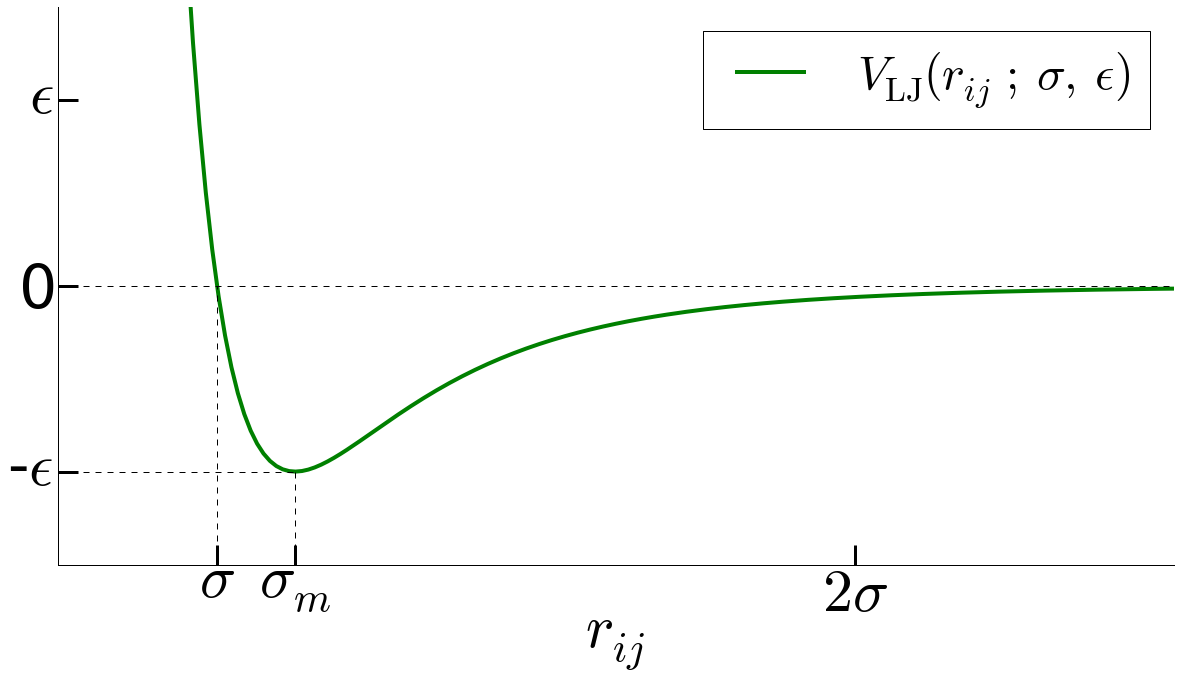
\includegraphics[width=0.7\textwidth]{LJ.png}}{./movies/simple2D_LJ_MINIMAL.avi}
\end{center}

\clearpage

%------------------------------------------------

\begin{center}
\movie[]{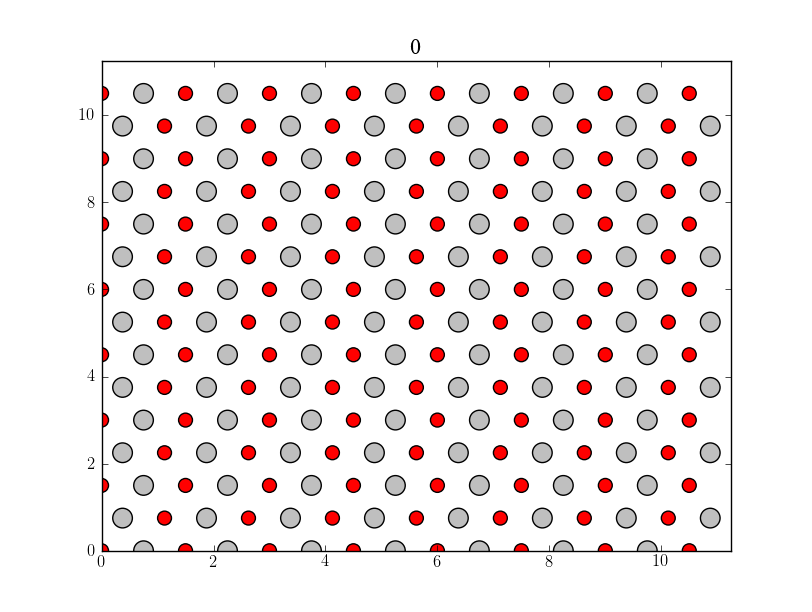
\includegraphics[width=0.7\textwidth]{./movies/mdPos00000_0.png}}{./movies/simple2D_LJ.avi}
\end{center}

\clearpage

%------------------------------------------------

\subsection{Why do we need quantum mechanics?}

\mybox{0.8\textwidth}{
\begin{itemize}
 \item Dramatically increases the \underline{predictive power} of MD.
\end{itemize}
}

\clearpage

%------------------------------------------------


\section{Introducing Quantum Mechanics}

\subsection{Difference from Newtonian Mechanics}

\clearpage

%------------------------------------------------

Imagine having a series of \textit{identical} experiments.

\mybox{0.8\textwidth}{
\begin{itemize}
 \item \textbf{Classical scale:} Every measurement yields the same result $\mathbf{m}_{\mathrm{CL}}$.
 \item \textbf{Quantum scale:}   Every measurement $\mathbf{m}_{\mathrm{QM}}$ can in theory be different, however, under the restriction that\\
 $\langle \mathbf{m}_{\mathrm{QM}} \rangle = \mathbf{m}_{\mathrm{CL}}$
\end{itemize}
}

\begin{center}
\movie[]{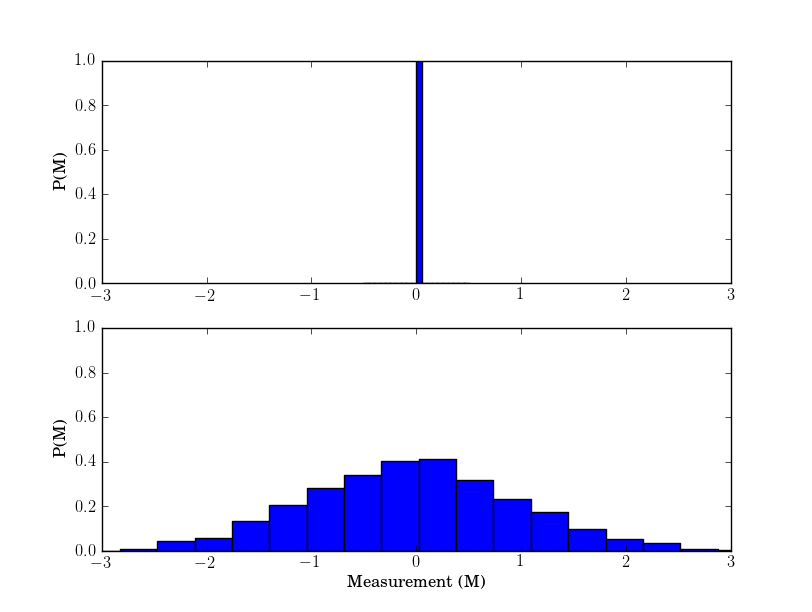
\includegraphics[width=0.7\textwidth]{./movies/FOR_PRESS_00051.png}}{./movies/clVsQmDist.avi}
\end{center}

\clearpage
%------------------------------------------------

If you have obtained this distribution of measurements, that is, you know the \textit{wave function}, you may calculate any \textit{observable} quantity related to the system.

\clearpage
%------------------------------------------------

In order to calculate the dynamics of a system we must ...

\mybox{0.8\textwidth}{
\begin{itemize}
 \item \textbf{Classical scale:} Solve Newton's second law for a given force field. Goal is to obtain a trajectory in phase space. 
 \item \textbf{Quantum scale:}   Solve Schr\"{o}dinger's equation for a given potential. Goal is to obtain the wave function.
\end{itemize}
}

\clearpage
%------------------------------------------------



\subsection{Challenges}

\clearpage

%------------------------------------------------

\subsubsection*{The electrons}

\begin{itemize}
\item  Not point particles as in classical theories.
\end{itemize}

\clearpage

%------------------------------------------------



\subsubsection*{The electrons}

\begin{itemize}
\item  Not point particles as in classical theories.
\item  A wave in space with given physical properties such as e.g.~mass and charge.
\end{itemize}

\clearpage

%------------------------------------------------



\subsubsection*{The electrons}

\begin{itemize}
\item  Not point particles as in classical theories.
\item  A wave in space with given physical properties such as e.g.~mass and charge...
\item  ... which implies interference with other electrons...
\end{itemize}

\clearpage

%------------------------------------------------

\subsubsection*{The electrons}

\begin{itemize}
\item  Not point particles as in classical theories.
\item  A wave in space with given physical properties such as e.g.~mass and charge...
\item  ... which implies interference with other electrons...
\item  ... which in turn implies that the solutions are not separable into single particle solutions.
\end{itemize}

\clearpage

%------------------------------------------------

The system needs to be treated as one unified entity; the electrons are \textit{entangled}.\\
\textit{Crucial} in order to describe chemical reactions and molecular structures.


\clearpage

%------------------------------------------------

\subsubsection*{The Computations}

\begin{itemize}
\item All differential equations become coupled, the CPU-time vs. system size scaling is off the charts.
\item Similar to Taylor polynomials, the more complex the system becomes, and thus the resulting wave function, the more basis elements we need to include to describe it well. Extreme scaling here as well.
\end{itemize}

\clearpage

%------------------------------------------------

\subsubsection*{All in all}

Due to entanglement, the quantum computations scale extremely bad with the number of electrons. However, the gain is that we are able to study chemical reactions and molecular structures \textit{ab-initio}.

\clearpage

%------------------------------------------------

  \captionsetup[subfloat]{labelformat=empty}
\begin{figure}
 \begin{center}
  \subfloat[$N=2$]{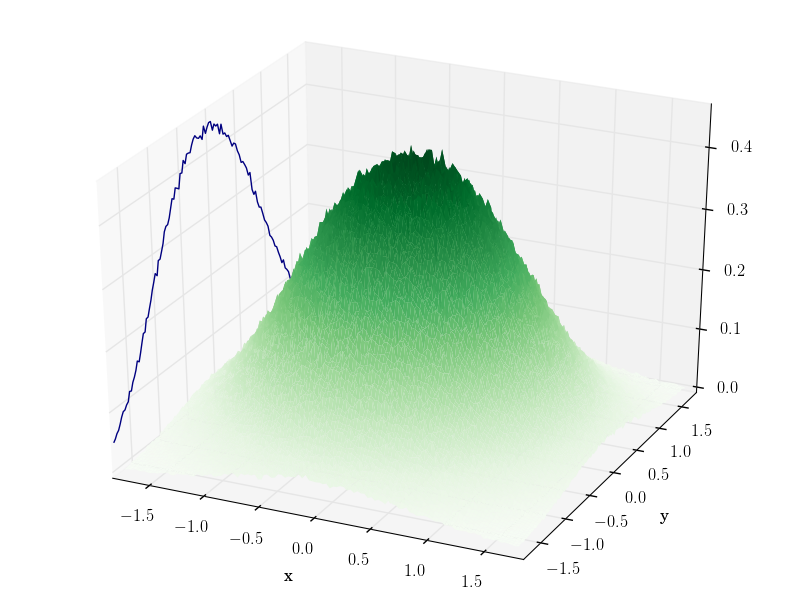
\includegraphics[scale=0.14]{graphics/OBD/dist_out_QDots2c1_3D.png}}
  \subfloat[$N=12$]{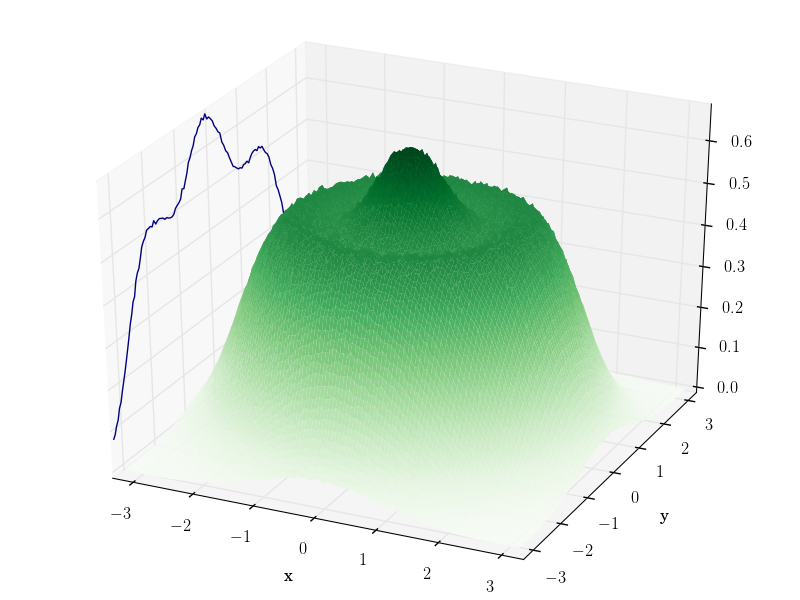
\includegraphics[scale=0.14]{graphics/OBD/dist_out_QDots12c1_3D.png}}
  \subfloat[$N=30$]{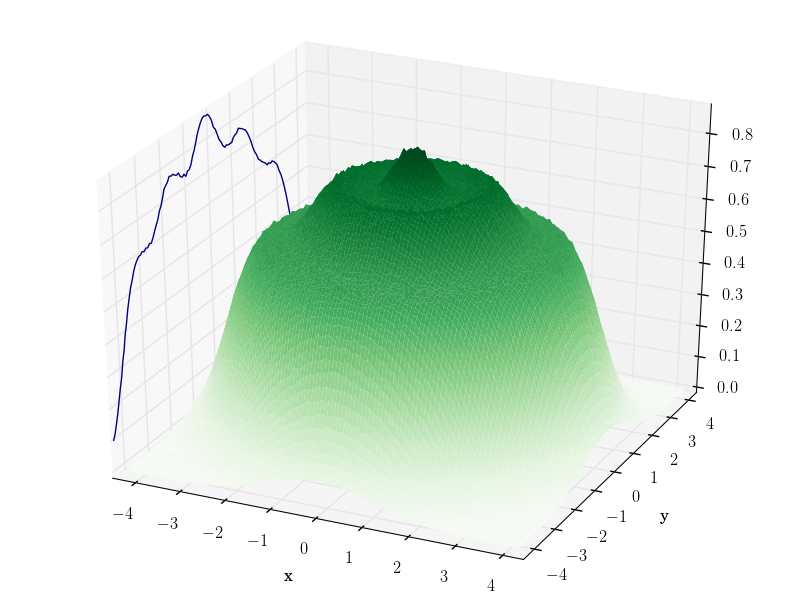
\includegraphics[scale=0.14]{graphics/OBD/dist_out_QDots30c1_3D.png}}\\
  \subfloat[$N=6$]{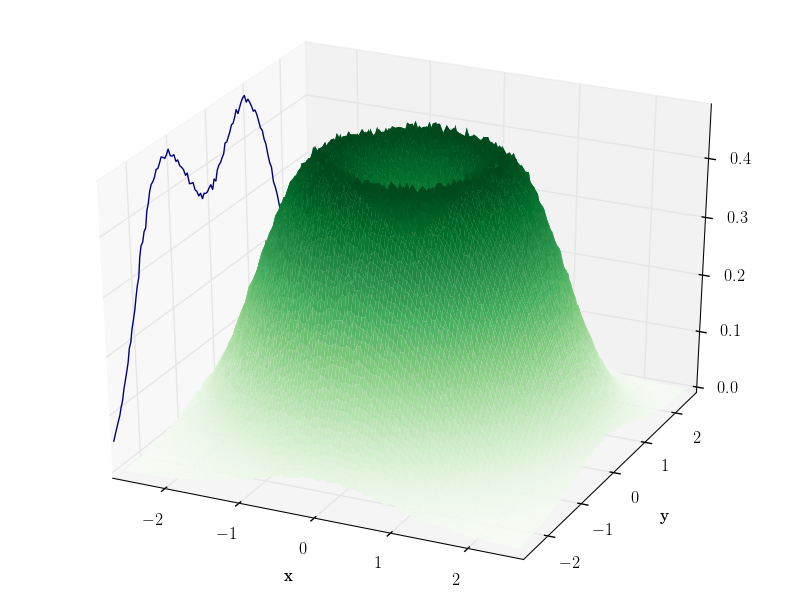
\includegraphics[scale=0.14]{graphics/OBD/dist_out_QDots6c1_3D.png}} 
  \subfloat[$N=20$]{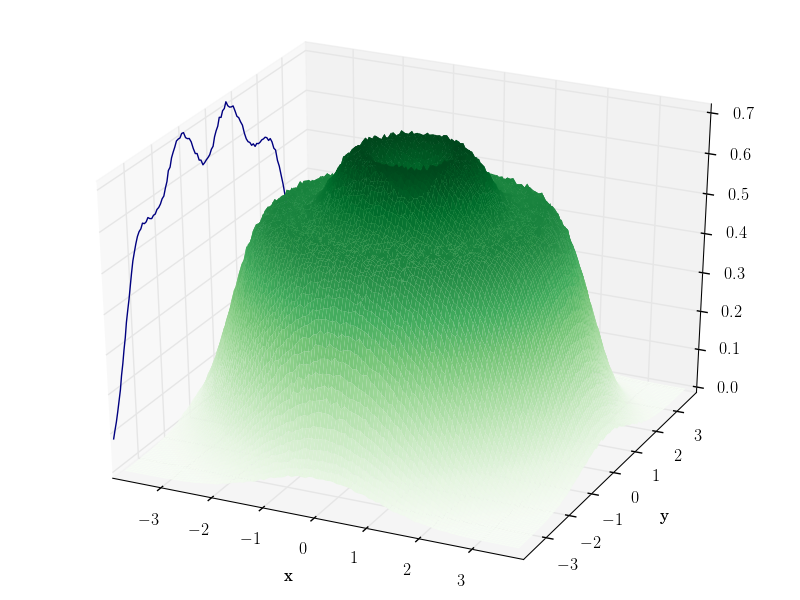
\includegraphics[scale=0.14]{graphics/OBD/dist_out_QDots20c1_3D.png}} 
  \subfloat[$N=42$]{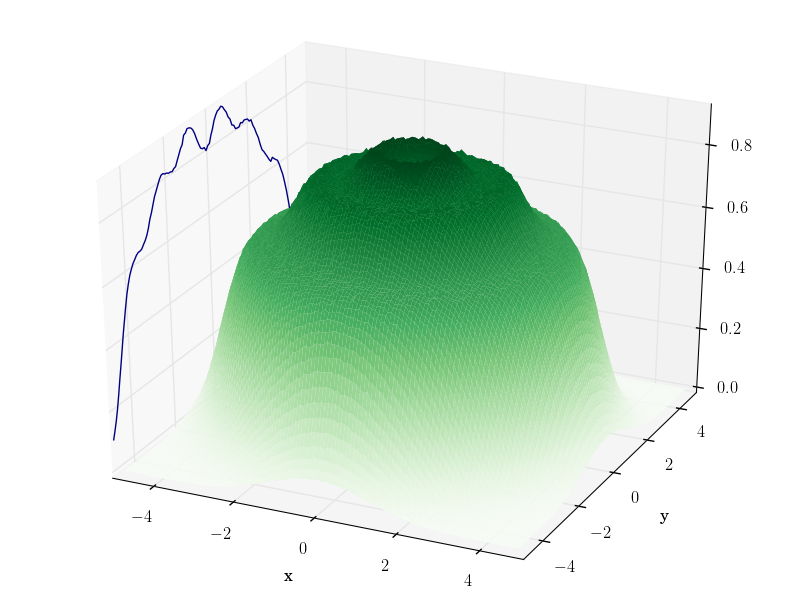
\includegraphics[scale=0.14]{graphics/OBD/dist_out_QDots42c1_3D.png}} \\
  \caption{\scriptsize{Densities for two-dimensional quantum dots.}}
  \label{fig:OBD_DMC_QDOTS_w1} 
 \end{center}
\end{figure}
\clearpage

%------------------------------------------------

When the electron density is lowered, we approach a limit where the quantum and classical solutions are reconciled. We \textit{un-entangle} the system.

\clearpage

%------------------------------------------------

 \begin{figure}
 \begin{center}
  \subfloat{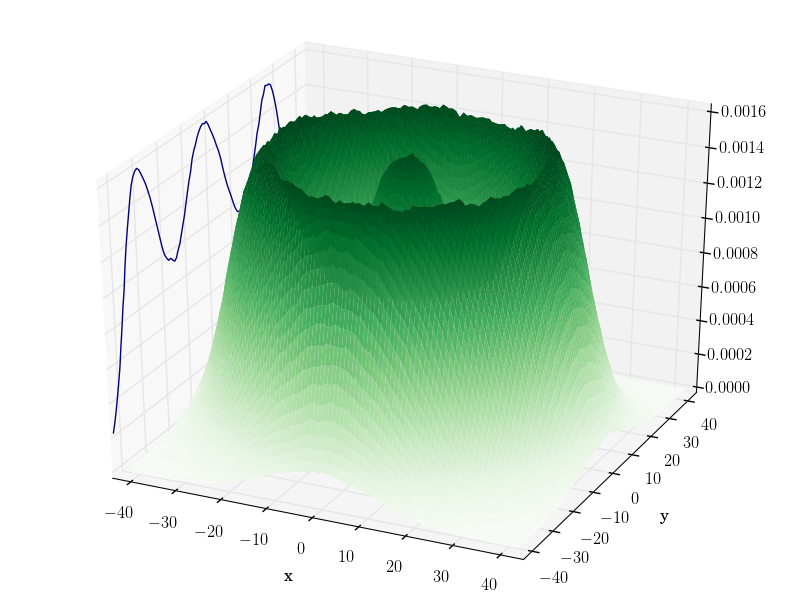
\includegraphics[scale=0.25]{dist_out_QDots6c001_3D.png}}
  \subfloat{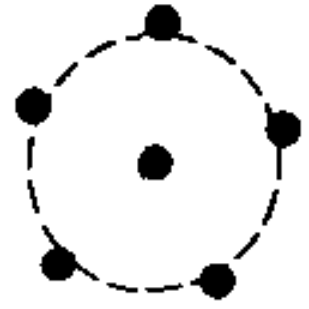
\includegraphics[scale=0.2]{wigner6.png}}
  \label{fig:wigner20}
  \caption{Density for a 6-particle two-dimensional quantum dot compared to the classical theoretical configuration taken from F. Bolton, U. R\"{o}ssler.  \textit{Superlattices and microstructures} \textbf{13}, 139 (1993).}
 \end{center}
\end{figure}

\clearpage

%------------------------------------------------

\section{Parameterizing Potentials using Quantum Mechanics}


\clearpage

%------------------------------------------------

\subsection{Connecting the scales}

How do we connect a molecular dynamics scenario of particle interactions to the quantum scale?

\clearpage

%------------------------------------------------

\begin{center}
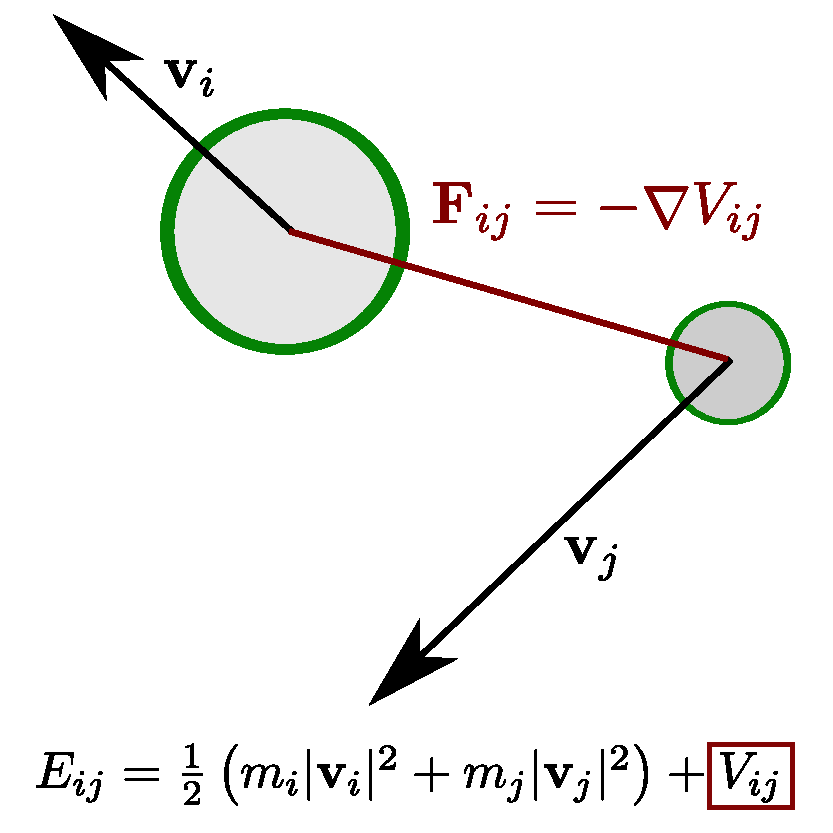
\includegraphics[width=0.55\textwidth]{moleculesColliding.pdf}
\end{center}

\clearpage

%------------------------------------------------

Let's freeze the dynamics as in the previous image and do some super advanced physics.
\clearpage

%------------------------------------------------

What is potential energy?
\clearpage

%------------------------------------------------
Well, it's what can be transferred into kinetic energy!
\clearpage

%------------------------------------------------
So, any energy sources that are \textbf{not} part of the MD kinetic energy is MD potential energy.
\clearpage

%------------------------------------------------

Since the electrons are not modeled in MD, kinetic energy of electrons count as potential energy in this case.
\clearpage

%------------------------------------------------

In other words: It is the total energy in quantum mechanics which corresponds to the potential in molecular dynamics.
\clearpage

%------------------------------------------------

Given a wave function for our system, e.g.~two molecules at a distance $r_{ij}$, the total quantum mechanical energy is obtained by calculating the expectation value of the \textit{Hamiltonian} $\mathbf{H}$

\mybox{0.9\textwidth}{
\begin{align}
 E_\mathrm{QM}(r_{ij}) &= \langle \mathbf{H} \rangle_{\psi(r_{ij})} \\
\mathbf{F}_{ij} &= -\nabla_{r_{ij}} E_\mathrm{QM}
 \end{align}
}

\clearpage

%------------------------------------------------


\subsection{Practical calculations}

\subsubsection*{Two-body forces}

Set up a model Hamiltonian for the scenario in the previous Figure:

\begin{itemize}
 \item Core-core Coulomb interaction.
 \item Electron-core Coulomb interaction.
 \item Electron-electron Coulomb interaction.
\end{itemize}


\clearpage
%------------------------------------------------

Benefits: One potential to rule them all.

\clearpage
%------------------------------------------------

$E_\mathrm{QM}(r_{ij})$ can be calculated for given values of $r_{ij}$ ($\mathbf{R}$ in the figure). The below figure shows calculations for $\mathrm{H}_2$

\begin{center}
 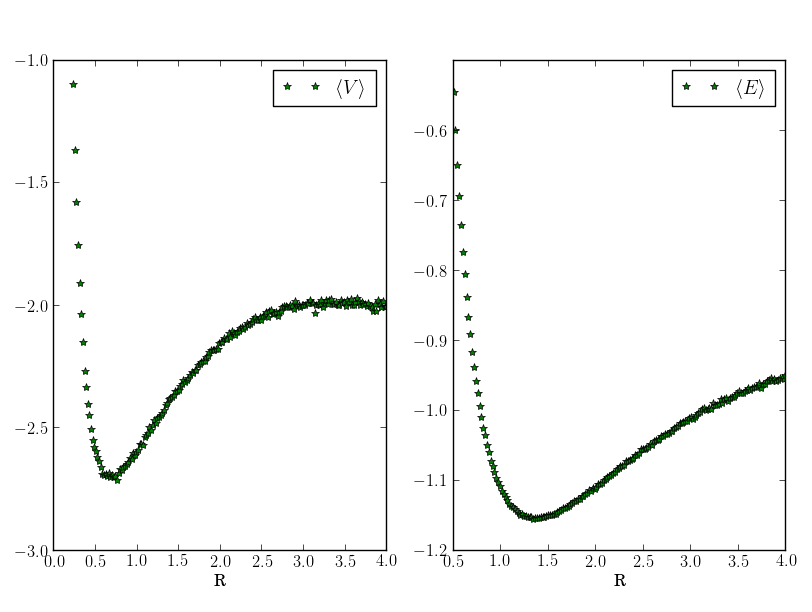
\includegraphics[width=0.6\textwidth]{R_vs_E_hyd_pure}
\end{center}


\clearpage
%------------------------------------------------

Studying the same calculations applied to $\mathrm{Li}_2$ we see something interesting...

\begin{center}
 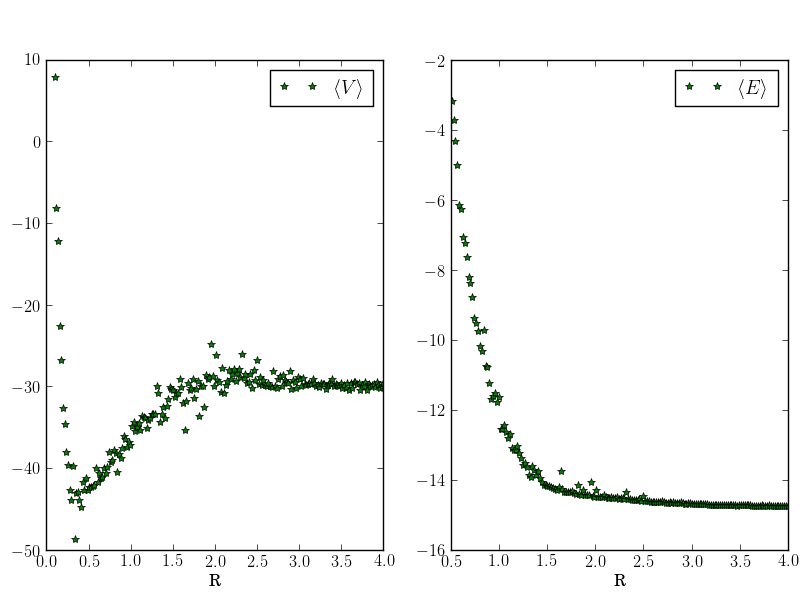
\includegraphics[width=0.6\textwidth]{R_vs_E_lit_pure}
\end{center}

\clearpage
%------------------------------------------------

Can this explain why di-litium isn't found in the universe?
\clearpage
%------------------------------------------------

\subsubsection*{N-body forces}

There is nothing which stands in the way for simulating as large of a system you want, however, keep in mind the terrible scaling.\\

In addition, for studying e.g.~silica structures, one would need a periodic system. Given entanglement \textbf{periodicity is non-trivial}. \\

One often settle with \textit{pseudo-periodicity} and approximative methods.

\clearpage
%------------------------------------------------

%------------------------------------------------
\subsection{State of the art}

Here I will discuss DFT, The nobel prize and so on. In addition I will mention some of the work done with e.g.~reaxff.

\clearpage


%------------------------------------------------

\thispagestyle{empty} % No slide header and footer

\begin{tikzpicture}[remember picture,overlay] % Background box
\node [xshift=\paperwidth/2,yshift=\paperheight/2] at (current page.south west)[rectangle,fill,inner sep=0pt,minimum width=\paperwidth,minimum height=\paperheight/3,top color=mygreen,bottom color=mygreen]{}; % Change the height of the box, its colors and position on the page here
\end{tikzpicture}
% Text within the box
\begin{flushright}
\vspace{0.6cm}
\color{white}\sffamily
{\bfseries\LARGE Questions?\par} % Request for questions text
\vfill
\end{flushright}

%----------------------------------------------------------------------------------------


\clearpage
$V_\mathrm{LJ}(r_{ij}\,;\,\sigma,\,\epsilon) = 4\epsilon \left(\left(\frac{\sigma}{r_{ij}}\right)^{12} - \left(\frac{\sigma}{r_{ij}}\right)^{6}\right)$


%----------------------------------------------------------------------------------------


\end{document}